\subsection{Networked Audio}\label{subsec:networked-audio}

The transmission of audio data has been a topic of research interest since the
earliest days of computer networking as it is recognised today, i.e.\ over
packet-switched networks, whereby data to be transmitted is grouped into
packets, each consisting of a header and a payload.
Voice transmission over ARPANET was being conducted as early as
1974~\citep{schulzrinne_voice_1992} and the first standard for voice
communication over packet-switched networks \textemdash{} the Network Voice
Protocol (NVP) \textemdash{} was released in
1977~\citep{cohen_specifications_1977}.

With its references to `calling' and `ringing', it is clear that the NVP
standard was intended for digital telephony.
Indeed, research on networked audio was primarily concerned with telephony well
into the 1990s, focusing on real-time voice communication over wide area
networks (WAN) with efforts centring on \textit{quality of service} (QoS),
particularly with regard to the perennial issues of latency, packet loss, and
network jitter \textemdash{} inconsistencies in the rate of packet
transmission~\citep{hardman_reliable_1995,hardman_successful_1998}.
Work at this time dealt with streams of compressed audio data, and speech
coding algorithms to overcome the deleterious effects of dropped packets over
unreliable network paths and low-bandwidth connections.

Whereas the priority for digital telephony, and later voice over IP (VoIP)
systems, is intelligibility, for musical purposes fidelity, and the use of
uncompressed audio signals, is of greater concern.
With the increasing availability of high-speed internet connections in the late
1990s came research into transmitting uncompressed audio data over the
internet~\citep{chafe_simplified_2000,xu_real-time_2000}.
Work of this sort was spearheaded by the \textit{SoundWIRE} project, developed
by researchers at McGill University and the Centre for Computer Research in
Music and Acoustics (CCRMA) at Stanford University, and took the form of
a wide variety of experiments with high quality audio over both WAN and local
area networks (LAN).
These experiments included LAN-based real-time musical
performances~\citep{chafe_simplified_2000}, concert streaming over
WAN~\citep{xu_real-time_2000,chafe_simplified_2000}, and sonification of QoS via
a distributed digital waveguide dubbed the
\textit{Network Harp}~\citep{chafe_simplified_2000,chafe_physical_2002}

\subsubsection{Protocols and Systems}\label{subsubsec:protocols-systems}

VoIP research in the 1990s focused on matters such as audio codecs and data
compression~\citep{turletti_inria_1995,hardman_successful_1998}, seeking a
compromise with the \textit{best-effort} nature of internet service.
The SoundWIRE project, in search of high audio quality, turned its attention
directly to the basic transport layer protocols of the Internet Protocol suite:
Transmission Control Protocol (TCP) and User Datagram Protocol (UDP).
Chafe et al.\ characterised their compression-free system as taking a
``simplified approach''~\citep{chafe_simplified_2000} to networked audio,
emphasising the importance of delivering multichannel audio of at least CD
quality (16-bit, \qty{44.1}{\kHz}) with as little latency as possible.

SoundWIRE experiments included using TCP for unidirectional transmission such as
concert streaming.
TCP is in fact a bidirectional protocol, but its \textit{connection-oriented},
one-to-one design, whereby networked entities establish a connection via a
`handshake', following which packets of data are exchanged, allows for
mechanisms that guarantee packet ordering and provide protections against packet
loss~\citep{schiavoni_alternatives_2013,al-dhief_performance_2018}.
These mechanisms mean that, at the expense of increased latency, quality of
service, and thus audio fidelity, is ensured; ideal for a remote concert
scenario.
%The strict one-to-one nature of TCP clearly places limits on its
%applicability to distributed computing, however.

UDP by comparison is a \textit{connectionless} protocol, providing no guarantees
regarding the integrity of the stream of network data, but equally none of the
computational, or indeed temporal, overhead that such guarantees introduce.
A network entity can send UDP packets to a network address irrespective of
the presence or otherwise of an entity at that address.
Further, \textit{many-to-many} (multicast) and \textit{one-to-many} (broadcast)
modes of transmission are possible via address spaces reserved as part of the
internet protocol standard~\citep{meyer_iana_2010}.
Via UDP, SoundWIRE was able to run as a distributed digital waveguide over a
WAN spanning around \qty{4500}{\km}~\citep{chafe_simplified_2000}.

From the SoundWIRE project emerged
\textit{JackTrip}~\citep{caceres_jacktrip_2010,caceras_jacktripsoundwire_2010},
a hybrid system that couples a TCP handshake with audio transmission over UDP,
thus sidestepping the overhead of TCP packet flow control.
Rather than relying on TCP's built-in mechanisms for stream integrity, JackTrip
supplements UDP with a number of optional buffering strategies that aim to
tailor its use to operation over local versus wide area networks.
In this sense it is more flexible than TCP, but in effect JackTrip moulds UDP
transmission into something akin to the connection-oriented model of TCP, and,
in its `hub server' mode, into a kind of \textit{multiple one-to-one} design
\textemdash{} multicast transmission is not possible.

UDP has emerged as the protocol of choice for platforms enabling remote musical
collaboration, serving as the basis for systems such as
NetJACK~\citep{carot_netjack_2009}, part of the JACK Audio Connection Kit (a
cross-platform audio host), Jamulus~\citep{fischer_case_2015},
Soundjack~\citep{renaud_networked_2012}, and other jamming-focused platforms,
plus more recent entrants such as the closed-source, but ultimately UDP-based
Elk OS~\citep{turchet_elk_2021}.
UDP even plays a fundamental role in proprietary systems such as Dante (Digital
Audio Network Through Ethernet)~\citep{noauthor_what_nodate}.

\subsubsection{AoE in the Audio Industry}

In parallel with the work being carried out by researchers such as those
developing SoundWIRE, JackTrip and NetJACK, audio industry bodies were taking
an interest in networked audio.
Prominent amongst these bodies were the IEEE (Institute of Electrical and
Electronics Engineers) and AES (Audio Engineering Society) standards groups,
and companies like Audinate, the creators of the Dante system.
Traditional large-scale audio systems such as those used in broadcast, concert
venues and recording studios rely on the installation of unwieldy systems of
analogue hardware and cabling, with many potential points of failure.
Seeking literally to lighten the load posed by ``hundreds of
kilograms''~\citep{bakker_introduction_2014} of analogue cabling in analogue
audio installations, in the 2000s industry entities were looking to high speed
ethernet as a means to simplify the provision of high-quality, multichannel
audio in industry settings.

Dante, with its promise of low-latency, highly-multichannel audio over ethernet,
and device synchronisation via Precision Time Protocol (PTP), has become the de
facto standard in this area~\citep{bakker_introduction_2014}.
In 2011, IEEE released the Audio Video Bridging (AVB, IEEE 802.1) standard,
and AES67 followed in 2013; these open technical standards describe operation
at layers below TCP and UDP in the OSI (Open Systems Interconnection)
model~\citep{}\todo[inline]{Add source for OSI}, and provide frameworks for
interoperability between AoE and AoIP systems, including mechanisms for device
discovery and synchronisation, again via PTP\@.
Being standards, and not implementations in themselves, it is then up to
manufacturers to implement the appropriate recommendations in their products.
(AES67, for example, has in fact been implemented in Dante.)

Bakker et al.\ refer to Dante as an ``open'' system.
This is perhaps true in the sense that companies can incorporate the Dante
system into their own products under licence from Audinate, but, from the
perspective of the academic community, Dante is very much a closed-source
initiative and not a suitable platform for research.
Open implementations of AVB and AES67 could be of interest, however their
reliance on PTP, support for which is not offered by ubiquitous, low-cost
networking equipment, raises the barrier to entry to systems based on these
standards.
Ultimately, if an accessible solution is sought, attention must be turned back
to the transport layer, and UDP\@.


\subsubsection{Anatomy of a Datagram}\label{subsubsec:anatomy-of-a-datagram}

\begin{figure}[h]
    \centering
    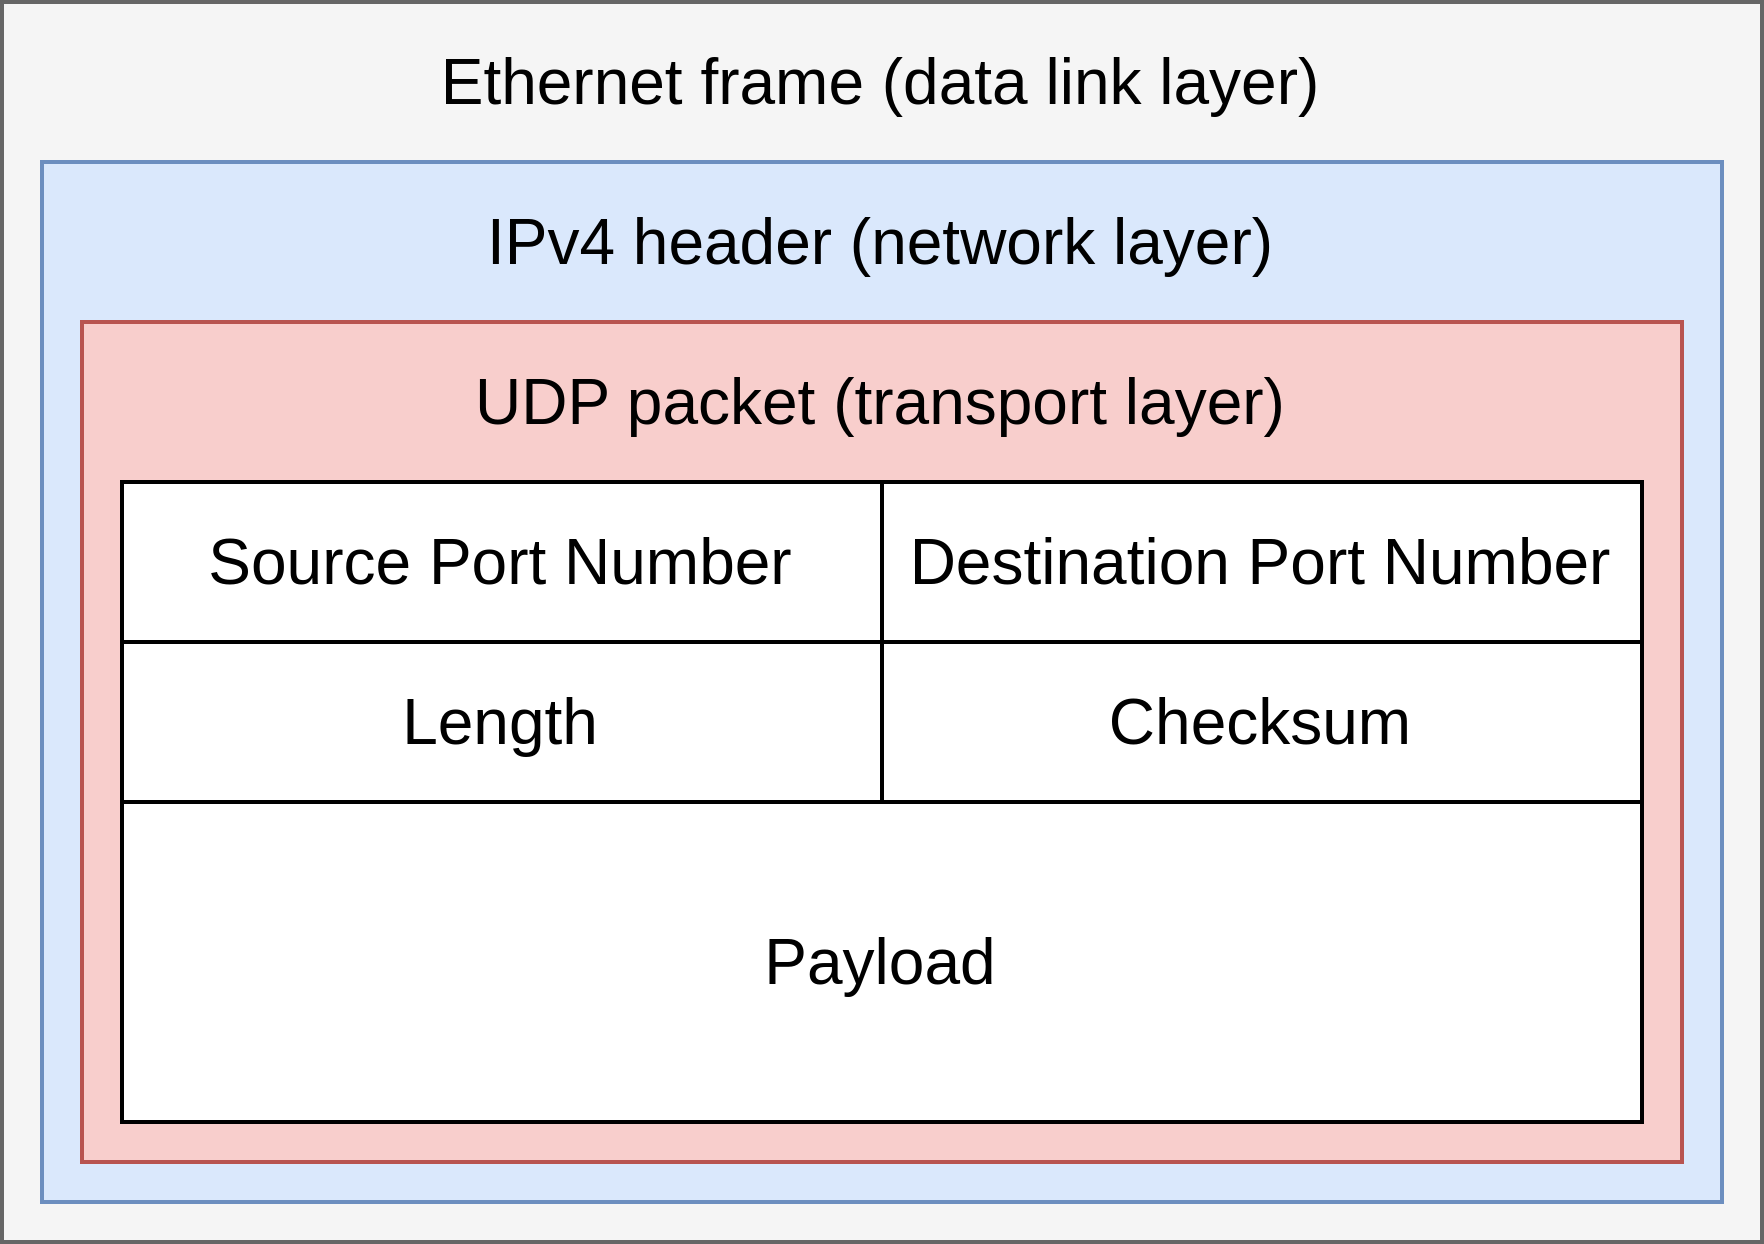
\includegraphics[width=.5\textwidth]{figures/udp}
    \caption{Structure of an ethernet frame containing a UDP packet.}
    \label{fig:udp-frame}
\end{figure}

A UDP packet consists of data encoded in 8-bit integer format.
Being a transport layer protocol, a UDP packet is in fact preceded in an
ethernet frame by information relating to lower layers in the OSI hierarchy: the
network layer and the data link layer.
The structure of a UDP packet (within an ethernet frame) is shown in
\figref{fig:udp-frame}.

\codeinputlisting[float=h]
{text}
{listings/udp-packet.txt}
{Network capture: ethernet frame containing a UDP packet}
{packet-hello-world}
\noindent
The ethernet frame in \lstref{listing:packet-hello-world} was generated
using the Netcat (\texttt{nc}) command line utility\footnote{
    \url{https://nc110.sourceforge.io/}
}, and captured with Wireshark network traffic analysis software.
Four-digit numbers to the left indicate the hexadecimal index of the byte
at the beginning of the corresponding line.
The central block of two-digit hexadecimal numbers are a representation of the
bytes in the ethernet frame, labelled above by byte position.
The block of characters to the right are the same data encoded as ASCII
characters.

\begin{table}[h]
    \centering
    \begin{tabular}[h]{c c c c}
        Start           & End             & Purpose                 & Value                                        \\
        \midrule[1pt]
        \texttt{0x0000} & \texttt{0x000d} & Ethernet header         &                                              \\
        \midrule
        \texttt{0x0000} & \texttt{0x0005} & Destination MAC address &                                              \\
        \texttt{0x0006} & \texttt{0x000b} & Source MAC address      &                                              \\
        \texttt{0x000c} & \texttt{0x000d} & Ethernet frame type     & \texttt{0x0800}: IPv4                        \\
        \midrule[1pt]
        \texttt{0x000e} & \texttt{0x0021} & IPv4 header             &                                              \\
        \midrule
        \texttt{0x0017} & \texttt{0x0017} & Protocol                & \texttt{0x11}: UDP                           \\
        \texttt{0x001a} & \texttt{0x001d} & Source IP address       & \texttt{0xac1efedf}: \texttt{172.30.254.223} \\
        \texttt{0x001e} & \texttt{0x0021} & Destination IP address  & \texttt{0x7f000001}: \texttt{127.0.0.1}      \\
        \midrule[1pt]
        \texttt{0x0022} & \texttt{0x0029} & UDP header              &                                              \\
        \midrule
        \texttt{0x0022} & \texttt{0x0023} & Source port number      & \texttt{0xed3f}: \numDec{60735}              \\
        \texttt{0x0024} & \texttt{0x0025} & Destination port number & \texttt{0x22b8}: \numDec{8888}               \\
        \texttt{0x0026} & \texttt{0x0027} & Length                  & \texttt{0x0016}: \numDec{22}                 \\
        \midrule[1pt]
        \texttt{0x002a} & \texttt{0x0037} & UDP Payload             &                                              \\
        \bottomrule
    \end{tabular}
    \label{tab:packet-structure}
    \caption{Description of selected fields in the UDP packet depicted in
    \lstref{listing:packet-hello-world}.}
\end{table}

Bytes \texttt{0x0000} to \texttt{0x000d} make up the ethernet header,
consisting of the media access control (MAC) addresses of the destination and
source; the final two bytes of the ethernet header, \texttt{0x0800}, indicate
that this is an \textit{internet protocol version 4} frame.
Bytes \texttt{0x000e} to \texttt{0x0021} are the IPv4 header; this contains
information about the internet protocol part of the packet, such as its length
in bytes \textemdash{} \texttt{0x002a} (\numDec{42}) \textemdash{} and
the source and destination IP addresses, encoded as groups of four-bytes.
The source IP address, for example, is \texttt{0xac1efedf}, a 32-bit encoding
of the more familiar-looking \texttt{172.30.254.223}.

Beginning at byte \texttt{0x0022} is the UPD header.
This contains the source port (\texttt{0xed3f}, \numDec{60735}), destination
port (\texttt{0x22b8}, \numDec{8888}), the length of the UDP part of the frame
(\texttt{0x0016}, \numDec{22} bytes) and ends with a checksum, which
can be used to verify the integrity of the packet\footnote{
    In the remainder of this work it is assumed that transmission over LAN is
    unlikely to result in packet corruption; the UDP checksum is not used.
}.
The packet payload begins at byte \texttt{0x002a}, and consists of bytes
corresponding with the ASCII characters \texttt{Hello, world!}, plus
\texttt{0x0a}, the line feed (LF) character, captured and sent by Netcat when
the user hit the return key.

Netcat takes data supplied to a computer's standard input stream, in this
case characters supplied to a terminal emulator, and uses this data as the
payload for the packet to be transmitted.
The payload of a UDP packet can of course consist of any data which can be
appropriately byte-encoded, such as a stream of audio samples, or audio control
data such as MIDI or OSC messages.

Ethernet frames, and UDP datagrams by extension, are subject to size
limitations.
The maximum transmissible unit (MTU) of a transport medium is the limit on the
size of a packet that can be sent without fragmentation, i.e.\ without being
split into multiple sub-packets.
Two bytes (sixteen bits) are allocated to the `Total Length' field of the IPv4
header, which suggests an MTU of $2^{16}-1=~$\num{65535} bytes;
in practice, however, the data link layer imposes a basic limit of \num{1500}
bytes on the payload of an ethernet
frame~\citep{schiavoni_alternatives_2013,noauthor_ieee_2018}.
